\documentclass[tikz,border=4pt]{standalone}
\usepackage[T1]{fontenc}
\usepackage{lmodern}
\usetikzlibrary{arrows.meta,positioning,fit,backgrounds}
\begin{document}
\sffamily
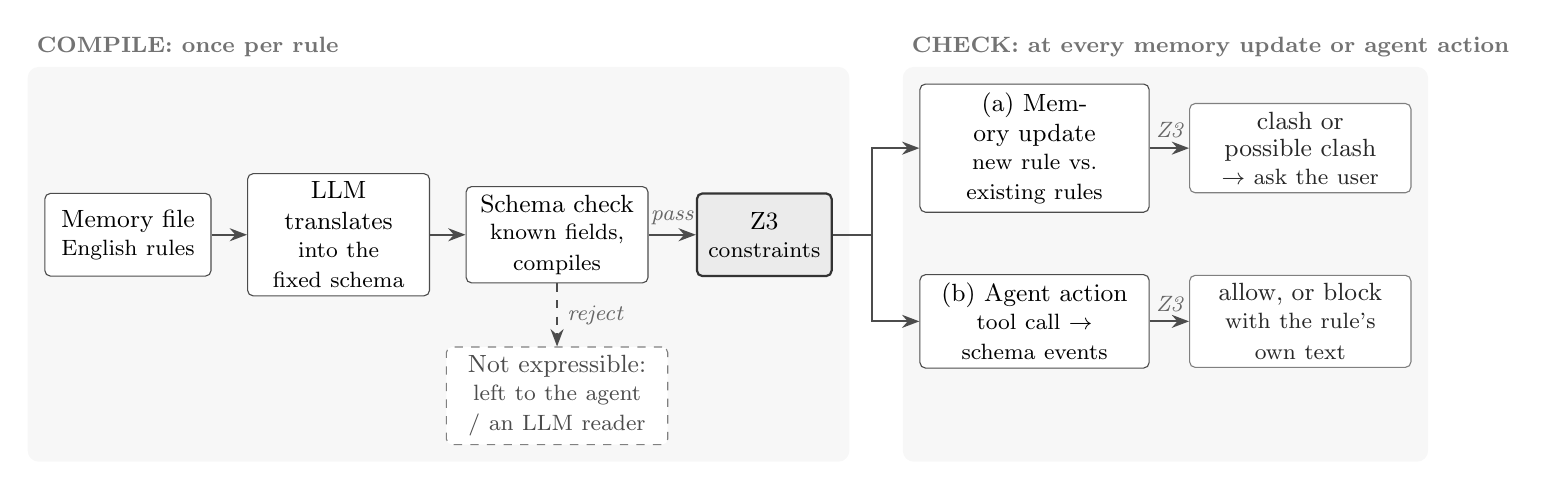
\begin{tikzpicture}[
  font=\small,
  box/.style={draw=black!70, rounded corners=2pt, align=center, minimum height=1.05cm, inner sep=3pt, fill=white},
  z3/.style={box, fill=black!8, draw=black!80, thick},
  res/.style={box, draw=black!50, text=black!85},
  side/.style={box, dashed, draw=black!50, text=black!70},
  arr/.style={-{Stealth[length=2.2mm]}, thick, black!70},
  lab/.style={font=\footnotesize\itshape, text=black!60},
  stage/.style={font=\footnotesize\bfseries, text=black!55}
]
% ---------------- compile once per rule
\node[box, text width=1.9cm] (mem) {Memory file\\[-1pt]\footnotesize English rules};
\node[box, text width=2.1cm, right=0.45cm of mem] (llm) {LLM translates\\[-1pt]\footnotesize into the fixed schema};
\node[box, text width=2.1cm, right=0.45cm of llm] (chk) {Schema check\\[-1pt]\footnotesize known fields, compiles};
\node[z3, text width=1.5cm, right=0.6cm of chk] (cons) {Z3\\[-1pt]\footnotesize constraints};
\draw[arr] (mem) -- (llm);
\draw[arr] (llm) -- (chk);
\draw[arr] (chk) -- node[lab, above] {pass} (cons);

\node[side, text width=2.6cm, below=0.8cm of chk] (rest) {Not expressible:\\[-1pt]\footnotesize left to the agent / an LLM reader};
\draw[arr, dashed] (chk) -- node[lab, right] {reject} (rest);

% ---------------- check every time
\node[box, text width=2.7cm, right=1.1cm of cons, yshift=1.1cm] (upd) {(a) Memory update\\[-1pt]\footnotesize new rule vs.\ existing rules};
\node[box, text width=2.7cm, right=1.1cm of cons, yshift=-1.1cm] (act) {(b) Agent action\\[-1pt]\footnotesize tool call $\to$ schema events};
\draw[arr] (cons.east) -- ++(0.5,0) |- (upd.west);
\draw[arr] (cons.east) -- ++(0.5,0) |- (act.west);

\node[res, text width=2.6cm, right=0.5cm of upd] (upd-out) {clash or\\[-1pt]possible clash\\[-1pt]\footnotesize $\to$ ask the user};
\node[res, text width=2.6cm, right=0.5cm of act] (act-out) {allow, or block\\[-1pt]\footnotesize with the rule's own text};
\draw[arr] (upd) -- node[lab, above] {Z3} (upd-out);
\draw[arr] (act) -- node[lab, above] {Z3} (act-out);

% ---------------- stage labels
\begin{scope}[on background layer]
  \node[fit=(mem)(llm)(chk)(cons)(rest)(upd.north -| mem), inner sep=6pt, fill=black!3, rounded corners=4pt] (s1) {};
  \node[fit=(upd)(act)(upd-out)(act-out)(rest.south -| upd)(upd.north -| upd), inner sep=6pt, fill=black!3, rounded corners=4pt] (s2) {};
\end{scope}
\node[stage, anchor=south west] at (s1.north west) {COMPILE: once per rule};
\node[stage, anchor=south west] at (s2.north west) {CHECK: at every memory update or agent action};
\end{tikzpicture}
\end{document}
